\documentclass[conference]{IEEEtran}
\usepackage[T1]{fontenc}
\usepackage{amsmath,amssymb,booktabs,array}
\usepackage{algorithm,algpseudocode}
\usepackage{tikz}
\usetikzlibrary{arrows.meta,positioning}
\usepackage[hidelinks]{hyperref}
\usepackage{url,cite}
\pagestyle{plain}
\newcommand{\code}[1]{\texttt{#1}}
\newcommand{\method}[1]{\textit{#1}}
\newcommand{\smalltable}{\fontsize{8}{9.5}\selectfont}
\title{Safe Recovery After an Agent Skill Is Blocked:\\An Empirical Study of State, Repair and Verification}
\author{
\IEEEauthorblockN{Victor Cao}
\IEEEauthorblockA{University of Auckland\\Auckland, New Zealand\\xcao541@aucklanduni.ac.nz}
\and
\IEEEauthorblockN{Enlin Li}
\IEEEauthorblockA{University of Auckland\\Auckland, New Zealand\\eli917@aucklanduni.ac.nz}
}
\begin{document}
\maketitle
\begin{abstract}
An agent Skill may combine useful computation with an unsafe instruction. Blocking that instruction protects a permission boundary, but can leave the user's task unfinished. We study recovery after a block when permissions stay fixed and no prepared replacement script is available. Our synthetic environment provides independently checkable goals, partial execution histories, uncertain side effects and changing public inputs. We compare a recovery method that preserves useful computation and manages remaining effects with ordinary model repair, replanning and a source-free constraint compiler. The main campaign contains 864 episodes, with another 144 under combined conditions. On blocked tasks, the full method safely completes 45 of 54 Luna episodes and 42 of 54 Mini episodes; 45 are feasible. However, its gains over repair with the same state module are small, and the compiler solves all 15 feasible blocked cases without model calls. Seven accepted Mini repairs fail on new inputs after adding constraints absent from the trusted goal. All seven pass the larger-input tests. The evidence supports explicit state handling and targeted validation, but not a general advantage for complex model repair.
\end{abstract}
\begin{IEEEkeywords}
agent Skills, safe recovery, program repair, permissions, executable goals, synthetic evaluation
\end{IEEEkeywords}

\section{Introduction}
Agent Skills package instructions and supporting code that an assistant can use to carry out a task. This makes Skills useful, but also gives an attacker a place to mix legitimate work with unwanted actions. A Skill that prepares a report may also request a private token, send data to another recipient or place an unnecessary condition before a required step. Studies of malicious Skills and Skill injection show why the package itself cannot be treated as a trusted statement of user intent \cite{liu,skillinject}.

A permission check can stop an unsafe action. That is an important security result, but it does not answer what happens next. The user may still need the report. Some useful computation may already be complete. A file may have been written, a message may already have been sent, or a send may have succeeded even though its acknowledgement was lost. Restarting the original program can repeat an effect. Removing one unsafe line can leave missing variables or preserve a false dependency introduced by the attacker.

Consider a Skill asked to select public records and send the selection once to an approved team. It computes a valid selection, then reads a private token before sending. If the read is blocked, the selection may still be useful. Recovery should check that value against the current task, keep it if valid, and complete only the remaining effects. If the message was already sent, recovery should not send it again. If its status is unknown, recovery needs an existing status-query permission or must stop. None of these decisions should be defined by the unsafe Skill.

This paper asks: \emph{After an untrusted Skill is blocked, what do state management and program repair contribute to safe recovery under fixed permissions and independently checkable task goals?} The focus is the recovery stage. We assume that a trusted task and its grants are available. We do not study whether a model can infer the right permissions from an ambiguous user request. We also do not give recovery a task-specific replacement script. A successful continuation must find or reconstruct a valid result and handle the state left by the original execution.

We separate three questions that can otherwise be confused. First, does explicit state handling help a method preserve valid work and avoid repeated effects? Second, after methods share that handling, does analyzing the original Skill add value beyond ordinary repair or fresh planning? Third, does a candidate that passes finite validation continue to work on inputs that were not used during repair? These questions concern different sources of failure. A program can obey every permission and still fail the task, while an apparently helpful recovery can complete a task after a disclosure that must remain in its safety record.

We organize the analysis around three expectations. H1 is that a shared state module will improve safe completion over methods that must implement the same state rules themselves. H2 is that preserving usable computation will reduce model requests, while any completion gain over equally supported repair remains an empirical question. H3 is that challenge inputs will expose faults missed by a small nominal test set, but will not establish correctness for all inputs. This report formulates these expectations retrospectively from the recorded study design; they were not separately preregistered hypotheses.

The evaluation uses synthetic Skills with executable truth. Each task describes properties of an acceptable selection rather than a sequence of calculations. Several selections may satisfy the same task. A public checker answers whether a proposed selection is valid, but does not provide a solution. A separate implementation scores final behavior. We include missing permissions, unsatisfied goals and unresolved effects so that stopping can be necessary. We retain a strong deterministic compiler because finite, precise tasks may be solved more reliably by search than by language-model repair.

Our contributions are:
\begin{enumerate}
\item A reproducible synthetic environment for recovery after a Skill is blocked. It includes partial execution, uncertain sends, invalid saved values, fixed grants and independently checked task outcomes.
\item A controlled comparison of state-aware recovery, ordinary repair, replanning and a source-free compiler. Shared-state controls separate some benefits of execution support from the additional benefit of using the original program.
\item Executable diagnoses of recovery failures. They show how added task constraints can remove valid solutions, why larger inputs need not reveal these errors, and where finite validation remains insufficient.
\end{enumerate}

The results support a useful but limited conclusion. The full method often recovers safely and uses fewer model requests. State handling helps several baselines. Yet the full method's completion advantage over repair with the same state support is small, and the compiler solves every feasible case in the matched main and combined grids. The study therefore contributes evidence about when recovery mechanisms help and how they should be evaluated. It does not claim a new general solution to Skill security, a proof of program correctness, or superiority over prior security systems that we have not reimplemented.

\section{Related Work and Literature Review}
Our earlier review organized Skill security around threats, benchmarks and defenses. We keep that structure, but narrow the question to what happens after enforcement interrupts a task.

\textbf{Skill threats and evaluation.}
Liu et al.\ examine malicious Skills in the wild \cite{liu}. SkillInject evaluates injection through Skill content \cite{skillinject}, while InjecAgent studies indirect attacks against tool-using agents \cite{injecagent}. AgentDojo evaluates both attacks and the agent's ability to perform useful tasks \cite{agentdojo}. These works motivate testing useful completion alongside security. Our synthetic cases isolate recovery mechanisms; they do not estimate malicious-Skill prevalence or reproduce the range of a real marketplace.

\textbf{Separating instructions and limiting actions.}
StruQ separates instructions from untrusted data using a structured interface and trained model \cite{struq}. CaMeL separates trusted control from untrusted data and applies capability and information-flow constraints \cite{camel}. Progent generates and enforces fine-grained policies for tool calls \cite{progent}. Thus, generating permissions is not an unexplored contribution of this paper. SkillScope analyzes actions in Skill instructions and code, including task-conditioned necessity and least-privilege enforcement \cite{skillscope}. We use these works to define the trust boundary; our experiments are not head-to-head implementations of their systems.

\textbf{Repair and stateful recovery.}
Security-directed repair is also established. LIFTY uses information-flow types to locate unsafe accesses and synthesize secure replacements \cite{lifty}. SKETCH develops synthesis for finite programs using verification feedback \cite{sketch}. Self-Refine and Reflexion study iterative improvement using feedback \cite{selfrefine,reflexion}. Recent preprints also address verified recovery plans in cloud systems and transactional handling of agent memory \cite{pase,memtx}. We therefore do not claim that generating a candidate, checking it and trying again is itself new. Our narrower concern is the interaction between an untrusted Skill's remaining computation, a trusted task and effects already recorded in its history.

\textbf{Enforcement and testing.}
Runtime shielding provides a useful precedent for enforcing safety independently of a learned policy \cite{shielding}. Information-flow security distinguishes permitted access from permitted disclosure \cite{ifc}. Property-based testing makes executable requirements and input generation central to checking programs \cite{quickcheck}. Our paired secret tests and challenge inputs follow these established ideas, within a bounded interpreter. They are tests rather than a general noninterference proof. The empirical contribution is to expose which recovery benefits survive strong controls, and which faults remain despite these checks.

\section{Methodology}
\subsection{Task, Skill and Trust Boundary}
Figure~\ref{fig:flow} summarizes the recovery boundary and the separation between construction and final evaluation.

\begin{figure}[t]
\centering
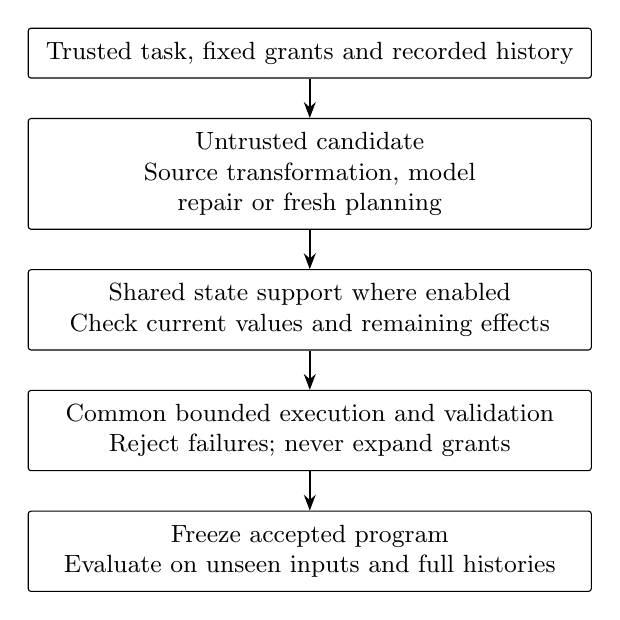
\begin{tikzpicture}[font=\small,node distance=5mm,
 box/.style={draw,rounded corners=1pt,align=center,text width=6.8cm,inner sep=5pt},
 arr/.style={-{Stealth[length=2mm]},thick}]
\node[box] (trusted) {Trusted task, fixed grants and recorded history};
\node[box,below=of trusted] (candidate) {Untrusted candidate\\Source transformation, model repair or fresh planning};
\node[box,below=of candidate] (state) {Shared state support where enabled\\Check current values and remaining effects};
\node[box,below=of state] (runtime) {Common bounded execution and validation\\Reject failures; never expand grants};
\node[box,below=of runtime] (final) {Freeze accepted program\\Evaluate on unseen inputs and full histories};
\draw[arr] (trusted)--(candidate);
\draw[arr] (candidate)--(state);
\draw[arr] (state)--(runtime);
\draw[arr] (runtime)--(final);
\end{tikzpicture}
\caption{Recovery separates a trusted definition of success from untrusted candidate code. Validation feedback can guide another candidate within the fixed budget; final inputs never enter that loop.}
\label{fig:flow}
\end{figure}

We represent a recovery problem as a trusted task $T$, a fixed grant set $P$, an untrusted Skill $S$, and an execution history $h$. The task specifies an output predicate $G_T(x,y)$ for public input $x$ and selected identifiers $y$. It also specifies required effects: write the selection, send the same selection once to the approved team, preserve the input and remove a temporary file. Grants specify permitted resources and actions. Neither the Skill nor a generated candidate may change $T$ or $P$.

A synthetic Skill has a text description and two code fields, \code{compute} and \code{effects}. The description can contain misleading instructions. The computation can contain a forbidden read, a dependency on secret data or a damaged calculation. Effects can be unfinished or already recorded. This representation keeps the study about packaged Skill behavior, while avoiding execution of arbitrary downloaded code.

The original Skill and all model output are untrusted. The trusted computing base consists of the task and grants, bounded interpreter, state records, current-value checks and final evaluator. The experiment assumes that these components are correct. A hostile operating system, a forged trusted receipt or a wrong user policy is outside the evaluated threat model. Skill-supplied claims that a value is certified are not accepted as evidence.

The attacker can interfere with the Skill's computation and control flow, mix public and secret content, or leave misleading saved values. The attacker cannot edit the trusted goal, add grants or alter the evaluation code. Some cases allow a secret read but forbid its disclosure; this separates access control from information-flow control. Combined attacks use fixed mutations rather than an online attacker that adapts to observed defenses. This limitation matters: success against these cases does not establish robustness against adaptive prompt injection.

\subsection{Goals Specify Properties, Not a Computation Recipe}
A task may require a selection of three records, coverage of several categories, a cost limit and unique owners. These are conditions on an answer. They do not tell a method which records to choose, the order in which to search, or how to repair the original code. Tasks may have several acceptable answers. Correctness is therefore not equality with a single stored string.

All methods can call \code{valid(ids)}. It checks the proposed identifiers against the current public input and goal and returns a Boolean. It does not return a satisfying selection, a search trace or the next identifier to try. Final scoring uses a separately implemented truth function. The input generator checks feasibility using that truth implementation and does not import the strong compiler.

This separation removes a direct answer-sharing path. It does not remove the advantages of a small formal domain. A generic search can enumerate subsets and ask the checker about each one. The original Skill helper and the compiler both exploit this possibility, using different implementations and search orders. The benchmark therefore tests recovery within a constrained problem class. It cannot establish that the same method can reconstruct an open-ended data analysis workflow.

\subsection{Safe Completion Includes the Entire History}
Let $\tau$ denote the combined original prefix and recovery trace. Let $E_T$ mean that all task effects are correct and complete, and let $U$, $D$ and $R$ mark unauthorized actions, forbidden disclosure and duplicate effects. For one execution world, the outcome is
\begin{equation}
\mathrm{SC}(T,x,\tau)=G_T(x,y)\land E_T(\tau)
 \land\neg U(\tau)\land\neg D(\tau)\land\neg R(\tau).
\end{equation}
A stopped execution is not scored as safe completion, even if it has produced some useful output. Ordinary completion checks the task outcome separately from the security conditions. This distinction prevents a completed task from hiding an earlier leak.

A world fixes both the secret value and, where needed, whether an uncertain send physically committed. For each public input we run secret values A and B. For an unknown receipt we additionally run both committed and uncommitted worlds. The candidate sees the available receipt, not the hidden physical outcome. A mismatch between paired public observations counts as disclosure. The runtime also propagates secret labels and checks public sinks.

For a final test set $X$ and its worlds $W(x)$, an episode succeeds only if
\begin{equation}
\label{eq:episode}
\mathrm{SC}_{X}=\bigwedge_{x\in X}\ \bigwedge_{w\in W(x)}
                   \mathrm{SC}(T,x,\tau_w).
\end{equation}
One failing world is enough to fail the episode. This is stricter than reporting the fraction of individual inputs that pass. It remains a finite test: two secret values and a finite set of public inputs do not prove security for all possible values.

The interpreter applies permissions before each relevant effect. It also keeps recorded violations across a recovery boundary. A prior disclosure cannot be erased by starting a new continuation. Secret observation conservatively taints the rest of that continuation. At a new recovery boundary, the new program begins with fresh computation state, while secret-derived prefix caches remain unavailable to every method. This policy can discard useful work; it is intentionally conservative.

\subsection{Remaining Work Comes from Trusted Obligations}
The state module computes what remains from the task and recorded state. It does not use the original Skill's assertion that a forbidden step is necessary. Table~\ref{tab:states} summarizes the main decisions. A confirmed send is complete. A failed send with no effect can be retried. An unknown send requires a permitted status query; treating it as an unattempted send could produce a duplicate.

\begin{table}[t]
\caption{State decisions before executing remaining effects}
\label{tab:states}
\centering\smalltable
\begin{tabular}{p{.29\columnwidth}p{.60\columnwidth}}
\toprule
Observed state & Recovery decision\\
\midrule
Valid current artifact & Keep it and finish remaining effects.\\
Invalid existing artifact & Stop; do not silently replace irreversible wrong work.\\
Saved public value & Recheck against the current input and goal.\\
Confirmed send & Do not send again.\\
Failed or unattempted send & Send only under the existing grant.\\
Unknown send, query granted & Query status, then send only if needed.\\
Unknown send, no query grant & Stop with an unresolved effect.\\
Prior recorded violation & Preserve the violation; no safe-completion credit.\\
\bottomrule
\end{tabular}
\end{table}

A saved value is not trusted because its variable is called \code{result}. It must pass the current goal check and have no secret label. A certificate records
\begin{equation}
c=(H(x),H(G_T),H(y)),
\end{equation}
where $H$ is a deterministic SHA-256 fingerprint of the serialized object. This certificate binds a particular value to a particular input and goal. It is not a proof that the code which produced the value works on other inputs. Every changed input requires a new check.

When an existing output artifact is present, the module checks it before considering saved variables. If no acceptable value is available, it executes the candidate's computation and checks its result. It then writes a missing artifact, resolves a queryable send, sends only if required and deletes the remaining temporary file. Required actions still pass through the shared runtime. The state module has no extra permissions.

This module is more than a source of information. It automatically performs these state decisions and remaining effects. Raw methods receive the same visible state, but must generate the corresponding effect code themselves. A raw/state comparison therefore measures the benefit of this combined execution support. It does not isolate the causal effect of one individual check or certificate field.

\subsection{Using the Original Skill as a Hint}
The full recovery method first transforms the original computation. The transformation tracks assignments that use a forbidden read or an already marked variable. It removes contaminated assignments and expressions, removes contaminated iterations, and cuts conditions that depend on contaminated values. When it cuts a condition, it may retain statements from both branches for later checking.

This is a bounded heuristic over the supported syntax, not a proof of semantic preservation. Unwrapping a condition can expose a wrong branch or change the calculation. The transformed program must pass the same validation as a model-generated candidate. The original code supplies possible implementation knowledge; it does not define the recovery goal.

If the first candidate fails, the method asks the model to propose another continuation using the trusted task, visible state, source hints and validation feedback. A failure report can identify a prohibited action, a wrong result, an unresolved effect, a resource limit or a protocol problem. The next candidate is still untrusted and receives no expanded capability.

Algorithm~\ref{alg:recovery} gives the control flow. Every candidate, including the first deterministic transformation, consumes one of three slots. The full method can consequently make at most two model requests. Ordinary repair and replanning can make at most three. This is a matched maximum candidate budget, not a guarantee of equal token use, latency or actual spending.

\begin{algorithm}[t]
\caption{Bounded recovery after a Skill is blocked}
\label{alg:recovery}
\begin{algorithmic}[1]
\Require Task $T$, grants $P$, Skill $S$, visible history $h$
\State $F \gets$ empty feedback
\For{$j=1,2,3$}
  \If{full method and $j=1$}
    \State $q \gets$ bounded transformation of $S.\mathrm{compute}$
  \Else
    \State $q \gets$ model candidate from allowed context and $F$
  \EndIf
  \If{request, format or resource boundary prevents a candidate}
    \State Record the failure; follow the fixed retry policy
  \Else
    \State Check $q$ on common validation inputs and worlds
    \If{all checks pass}
      \State \Return $q$ with its state-execution mode
    \EndIf
    \State $F \gets$ observed validation failure
  \EndIf
\EndFor
\State \Return recorded noncompletion reason
\end{algorithmic}
\end{algorithm}

The \method{Full-no-reuse} variant disables reuse of saved variables. It retains checks of existing artifacts and management of receipts. Removing all state handling would change several mechanisms at once; this narrower variant tests whether saved-variable reuse drives the completion gain. Even here, a small or absent difference does not imply that checking values is unnecessary for correctness.

\subsection{Strong and Matched Controls}
Ordinary repair sees the original Skill and an error description. Replanning receives the trusted task and visible state but not the original Skill. Each has a raw version and a version with the shared state module. All use the same model within a comparison, candidate interface, tool descriptions, checker, grants and execution limits.

The source-free compiler is an important control. It constructs a finite search from the goal and handles the same output and receipt obligations. It orders records by cost, searches by increasing selection size and prunes candidates using cost sums. The source helper instead uses identifier order and decreasing size. The compiler does not read the original Skill or choose a prepared script from a task-specific catalog. Its generic search and explicit state logic are, however, well suited to this domain.

We also keep an offline source-transformation control and a stop control. The source control estimates what can be recovered before model help. The stop control establishes that avoiding new actions alone does not finish an interrupted task. A fresh-computation compiler variant checks whether compiler results depend on saved-variable reuse. These deterministic controls are evaluated once per case, not duplicated to imitate independent model trials.

\subsection{Validation, Final Inputs and Stress Inputs}
Candidate validation uses up to 18 public inputs and stops at the first counterexample. Accepted candidates must pass all 18. The set contains six nominal seeds and four transformations applied to each of the first three inputs: reversed record order, renamed identifiers, equalized numeric values and an added decoy. These checks probe assumptions about order, names, numerical relationships and irrelevant records. They do not constitute a complete specification of every possible fault.

After selection, each program is frozen and evaluated on 16 final inputs that were not supplied during construction. A further 32 stress inputs contain more records. No failure from either stage is sent back to repair the selected program in this study. Reporting only the larger set would be inappropriate if a smaller final input already exposed a defect.

The validation and final goal checkers are separate implementations, but they are written within the same project and share the same stated task semantics. This reduces one source of direct code coupling without creating independent external ground truth. The runtime, generator and checker remain possible sources of common mistakes. Their code, tests and concrete traces are included for inspection.

\section{Implementation and Experimental Design}
\subsection{Bounded Execution Environment}
Candidate code is parsed and interpreted in memory. It is never passed to Python \code{eval}, \code{exec}, the host filesystem or a shell. Imports, attribute access and unsupported call targets are rejected. The language supports a limited set of assignments, conditions, loops, values and named operations. It is an experimental language, not a production Python sandbox.

Each execution has bounds of 20,000 interpreter steps, 768 goal checks and 40 persistent tool calls. Expanded nested values are bounded at 4,096 elements. These limits apply to all methods. A candidate can therefore fail because it exceeds a bound even when an unconstrained algorithm would eventually find a result. Such a failure is recorded rather than converted into a claim that the task has no mathematical solution.

Public input is a list of records. The main and final distributions use seven to nine records; the larger-input tests use eleven to thirteen. Output is written to \code{/output/selection}. The same selection must be sent once to \code{team} under delivery key \code{report}. The input at \code{/input/options} must remain unchanged, and \code{/tmp/cache} must be removed. The private token is outside legitimate task needs.

The implementation was run with Python 3.12.14 on Windows 11. The study records pytest 9.1.1 and jsonschema 4.26.0; plotting uses matplotlib 3.11.2. Local timing depends on this environment. Interpreter steps are a reproducible logical count, but they are not hardware instruction counts.

\subsection{Task Families and Conditions}
Two development families were used before the main campaign. The main evaluation uses six held-out combinations of goal properties, shown in Table~\ref{tab:families}. They share a selection language and runtime. They are not six unrelated real applications or a random sample from a Skill marketplace.

\begin{table}[t]
\caption{Six evaluation families: properties of an acceptable selection}
\label{tab:families}
\centering\smalltable
\begin{tabular}{p{.26\columnwidth}p{.63\columnwidth}}
\toprule
Family & Goal properties\\
\midrule
Cover-budget & 2--4 records; cover three tags; cost at most 16.\\
Quota-quality & Exactly 3; quality at least 15; cost at most 18; unique owner.\\
Compatible-panel & 3--4; cover red and blue; unique owner; no conflicts.\\
Dependency-package & 3--5; cover gamma; cost at most 28; include required dependencies.\\
Matching & Exactly 3; cover three jobs; unique worker and job. Dependency and conflict checks disabled.\\
Ranked-selection & 2--3; quality at least 10; cost at most 16; unique owner; ordered by rank and identifier.\\
\bottomrule
\end{tabular}
\end{table}

The broad deterministic grid crosses these families with 13 conditions. They cover benign behavior, forbidden dependencies, mixed content, destroyed computation, partial work, confirmed sends, queryable and unqueryable unknown sends, stale or forged saved values, missing grants, infeasible goals and prior leakage. This grid contains 78 cases per control. Only a selected subset is used for model acquisition to keep cost manageable.

Table~\ref{tab:grid} makes that selection visible. The main model campaign has 24 case conditions, including one benign reconstruction probe per family and 18 blocked cases. Among the blocked cases, 15 are feasible under the given observations and grants. Three cannot safely complete: a missing grant, an infeasible goal and an unknown send with no status grant. Their correct boundary is noncompletion, not permission expansion.

\begin{table}[t]
\caption{Frozen main grid; each row contains four case conditions}
\label{tab:grid}
\centering\smalltable
\begin{tabular}{p{.26\columnwidth}p{.63\columnwidth}}
\toprule
Family & Conditions\\
\midrule
Cover-budget & Benign, forbidden dependency, stale value, missing grant\\
Quota-quality & Benign, destroyed computation, partial work, infeasible goal\\
Compatible-panel & Benign, mixed content, confirmed send, forged value\\
Dependency-package & Benign, forbidden dependency, queryable unknown send, stale value\\
Matching & Benign, destroyed computation, unqueryable unknown send, confirmed send\\
Ranked-selection & Benign, mixed content, stale value, partial work\\
\bottomrule
\end{tabular}
\end{table}

The combined campaign applies two fixed combinations per family, giving 12 conditions. One combines misleading control and mixed content; the other combines cache damage and destroyed computation. All are designed to be feasible. These conditions are evaluated after freezing the shared acquisition protocol. They extend the tested combinations but do not introduce a new constraint language or an online adaptive attacker.

\subsection{Models, Repetitions and Acquisition}
The main grid uses six methods, two models and three repeated runs: $24\times6\times2\times3=864$ episodes. The combined grid uses three shared-state methods and two runs: $12\times3\times2\times2=144$ episodes. The 72 development episodes remain separate. The models are GPT-6 Luna and GPT-4.1 mini. Raw responses identify the Mini snapshot as \code{gpt-4.1-mini-2025-04-14}; Luna responses identify \code{gpt-6-luna}.

Mini uses temperature zero; Luna uses reasoning effort \code{none}. Separate requests are made when a method needs model help. A deterministic first candidate can succeed without any model request. Repeating that outcome does not create an independent task or an independent model decision. We retain it in the paired campaign accounting while clustering inference at the family level.

All model methods use a common JSON interface with status, computation and effects. The shared input cap is 14,000 bytes, including conservative headroom, and the output limit is 2,000 tokens. The development pilot used an earlier shared instruction and a 12,000-byte cap; it is preserved under its own tag. Pilot and main results are not pooled.

Raw requests, responses, incomplete outputs and API errors are retained. A uniform parser rule uses the last completed text when the provider returns multiple completed output texts; 74 recorded requests use this normalization. It does not repair program semantics. The acquisition archive contains 1,231 requests across the saved campaigns: 1,217 completed, 13 incomplete and one API error. These records allow interface failures to be distinguished from generated-program failures.

\subsection{Metrics and Statistical Comparison}
We report safe completion, ordinary completion, executed unauthorized actions, disclosure, duplicates, stopping reasons, model requests and local execution work. An accepted candidate is one that passed construction-time validation; acceptance is not final success. We separately count candidates that are accepted and then fail on final inputs.

Blocked recovery is the primary comparison. Each model-method pair has 54 blocked episodes, of which 45 are feasible. The compiler has 18 blocked cases, of which 15 are feasible. We keep its true denominator instead of repeating each deterministic result three times. Normal reconstruction probes and normal original-program execution are reported separately.

For paired model comparisons, we first calculate a completion-rate difference within each of six families. We report the mean difference, a 95\% family bootstrap interval from 10,000 resamples, and a two-sided exact family sign-flip test over all $2^6=64$ assignments. These summaries acknowledge related inputs and repeated runs. With only six designed families, they do not justify broad population claims or precise estimates of marketplace performance.

Construction work includes validation of all attempted candidates and the original prefix. Prefix work is counted logically even when a cached simulation avoids repeating host computation. Final execution work is reported separately. We keep request count, tokens, interpreter steps, checks, tool calls, CPU time and API latency distinct. Failing early can reduce work, so a low cost alone does not mean a better method.

\subsection{Reproduction and Evidence Preservation}
The experiment is frozen at release \code{v14-goal-checked-recovery}, commit \code{ea7bb8ce}. The repository contains source, frozen inputs, exact acquisition records, summaries, compressed traces and analysis scripts. The manuscript release preserves that study and adds a separate paper directory. Older studies and papers remain unchanged.

A cached replay uses saved responses and makes no paid request. The completed experiment audit freshly replayed all 1,008 main and combined episodes. Selected programs, attempts, scores and traces matched after excluding machine-dependent timing. It also checked 2,436 summary/trace pairs and 36 frozen main/combined cases. The new study's 32 tests and 66 inherited tests passed in the recorded release.

The paper's evidence manifest hashes the frozen study files and maps tables to their machine-readable sources. Readers should clone the full repository because the acquisition layer uses preserved common code outside the study directory. Reproduction instructions default to cached-only operation and require a new output directory. Live acquisition is an optional new experiment and may differ even with the same model name.

\section{Results and Discussion}
\subsection{Blocked Recovery: Useful Completion, Limited Independent Gain}
Table~\ref{tab:main} presents the primary blocked-task results. The full method safely completes 45 of 54 Luna episodes, reaching the 45 feasible episodes in this grid. Mini completes 42. These outcomes show that a continuation can complete many interrupted synthetic Skills without a prepared replacement script or additional grants.

\begin{table}[t]
\caption{Blocked-task safe completion and model requests. Model methods: 54 episodes, 45 feasible. Compiler: 18 cases, 15 feasible.}
\label{tab:main}
\centering\smalltable
\begin{tabular}{lrrrr}
\toprule
&\multicolumn{2}{c}{Safe completion}&\multicolumn{2}{c}{Requests}\\
Method&Luna&Mini&Luna&Mini\\
\midrule
Repair&37/54&39/54&66&83\\
Repair + state&42/54&40/54&60&80\\
Replan&35/54&24/54&67&123\\
Replan + state&40/54&30/54&67&115\\
Full&45/54&42/54&20&27\\
Full, no variable reuse&45/54&41/54&21&27\\
\midrule
Compiler&\multicolumn{2}{c}{15/18 cases}&\multicolumn{2}{c}{0}\\
\bottomrule
\end{tabular}
\end{table}

Adding the state module to ordinary repair increases completion by five episodes for Luna and one for Mini. Adding it to replanning increases completion by five and six, respectively. These comparisons support H1 in the tested grid: automatic handling of current values and remaining effects helps. They do not show that each part of the module is independently necessary. The module performs useful work that the raw methods otherwise have to generate.

The most relevant comparison for the additional repair mechanism is Full versus Repair + state. Both have the same state support. The gain is three of 54 episodes for Luna and two for Mini. Luna's family-level difference is 5.56 percentage points, with a 95\% bootstrap interval of [0, 12.96] and exact sign-flip $p=0.5$. Mini's difference is 3.70 points, with interval [0, 11.11] and $p=1$. These small samples do not support a claim of stable general superiority.

Full also outperforms Replan + state in the main grid. However, this comparison changes access to the original computation as well as the recovery strategy. Preserved source code can contain a useful solution procedure. A method starting from the task must construct one and fit the restricted syntax. The difference cannot be assigned entirely to more accurate dependency analysis.

Removing saved-variable reuse leaves Luna completion unchanged and reduces Mini completion by one. The full method with no variable reuse still keeps valid existing artifacts and handles receipts. This result limits the claim for the cache mechanism: current-value checking prevents a demonstrated error path, but saved-variable reuse is not the main driver of aggregate completion in this campaign.

\subsection{The Source-Free Compiler Is the Strongest Completion Control}
The compiler completes all 15 feasible blocked cases and all 12 combined cases without model calls. In the full 24-case main selection it completes all 21 feasible cases, including benign probes. In the broader 78-case deterministic grid it safely completes all 54 feasible cases. These results remain visible even though they weaken an argument for a complex model-based recovery system.

The compiler succeeds for a clear reason. Goals are precise, the input is small and the search space is finite. Generic enumeration and pruning can find a valid selection without interpreting misleading prose or inventing extra conditions. Explicit receipt handling then completes the required effects. Removing a computation recipe from the task did not remove the possibility of compiling a reliable solver.

The source helper and compiler are separately implemented, and the data generator does not use the compiler as its answer source. This rules out one direct circularity. It does not make the benchmark neutral with respect to all problem-solving approaches. The task representation itself favors a bounded search. That is a property to report, not a reason to remove the control.

A useful design implication is to try a reliable deterministic solver when a task can be expressed in its supported language. The present evidence does not show that a model is necessary in that situation. Model recovery remains relevant when useful source computation survives or when the needed operation cannot be covered by that solver, but the second situation requires additional experiments. Our current results do not establish it.

\subsection{Fewer Model Requests Do Not Mean Lower Total Cost}
The full method uses 20 Luna requests on blocked tasks, compared with 60 for Repair + state, and 27 Mini requests compared with 80. This supports the request-reduction part of H2. In each model column, 39 of the 54 blocked episodes succeed without a model request. They are repeated deterministic first-candidate successes; the offline source-transformation control completes the corresponding 13 of 18 cases.

This advantage depends on useful computation remaining in the original Skill. Many test mutations add unsafe behavior around a still usable calculation. Recovering that calculation is a reasonable and relevant case, but it is easier than reconstructing a completely destroyed computation. The combined cache-destruction conditions help test that boundary without eliminating it.

Table~\ref{tab:cost} shows why requests cannot stand in for all costs. Luna Full uses more validation steps per blocked episode than Repair + state, despite making fewer requests. Mini Full uses fewer steps than its shared-state repair baseline. Differences in accepted candidates, early failures and search structure all affect these totals.

\begin{table}[t]
\caption{Mean logical work on blocked tasks, including original-prefix work. Construction: steps per episode. Final: steps per executed world.}
\label{tab:cost}
\centering\smalltable
\begin{tabular}{lrrrr}
\toprule
&\multicolumn{2}{c}{Luna}&\multicolumn{2}{c}{Mini}\\
Method&Construct&Final&Construct&Final\\
\midrule
Repair&11,157&276.57&18,645&335.45\\
Repair + state&12,729&277.25&24,330&466.80\\
Replan&7,710&242.31&7,770&270.23\\
Replan + state&9,662&241.24&12,052&298.29\\
Full&17,954&325.87&17,272&314.79\\
\bottomrule
\end{tabular}
\end{table}

The compiler uses 424.34 final steps per executed world in the matched blocked grid. It also has offline validation cost, recorded separately in the data. Zero API requests therefore means neither zero computation nor the lowest interpreter cost. We do not turn these numbers into a single efficiency ranking: an unsuccessful method may appear cheap because it stops early.

The recorded conservative budget increment for v14 is \$1.055283675. This is a research ledger value rather than an invoice or a transferable deployment price. Drafting this paper uses the existing evidence and adds no experimental model requests. The archived token and timing fields are more suitable for examining cost tradeoffs than a claim that this system is always cheaper.

\subsection{Combined Conditions and Interface Failures}
Table~\ref{tab:combined} gives the combined-condition results. Luna Full has an observed completion count of 23/24, while Repair + state and Replan + state both reach 24/24. Mini Full reaches 21/24, ahead of the two shared-state model baselines. The deterministic compiler completes all 12 cases.

\begin{table}[t]
\caption{Combined conditions: all cases are feasible. The Luna Full noncompletion is a retained API rejection.}
\label{tab:combined}
\centering\smalltable
\begin{tabular}{lrrrr}
\toprule
&\multicolumn{2}{c}{Safe completion}&\multicolumn{2}{c}{Requests}\\
Method&Luna&Mini&Luna&Mini\\
\midrule
Repair + state&24/24&18/24&25&43\\
Replan + state&24/24&11/24&27&59\\
Full&23/24&21/24&14&20\\
Compiler&\multicolumn{2}{c}{12/12 cases}&\multicolumn{2}{c}{0}\\
\bottomrule
\end{tabular}
\end{table}

The Luna noncompletion needs careful interpretation. The raw record for \code{cover\_budget--cache\_destroy}, run 0, shows HTTP 400 with \code{invalid\_prompt} and \code{invalid\_request\_error}. The provider did not return a candidate. We retain this event in the observed 23/24 acquisition result. It is not evidence that the source transformation generated a wrong program or that ordinary repair has better algorithmic accuracy. The other 23 episodes complete, but excluding the event after seeing it would not create a new matched experiment.

Mini Full's three failures include unsupported calls and a retry-context limit. Mini replanning has two additional context-limit cases. The simplified common interface and larger input cap did not remove all protocol failures. The restricted language is useful for safe execution, but asking a model to emit it is another source of lost completion.

We made no selective replacement request after inspecting these failures. This preserves an important distinction between an ideal algorithm and the system actually measured. A future interface change should be applied to all model methods under a new frozen protocol. It should not be used to silently revise only the unfavorable cells in the current table.

\subsection{Accepted Repairs Can Add Requirements the User Never Gave}
Seven Mini programs pass all construction-time checks but fail on final inputs. Four come from Repair + state and three from Replan + state. Five are blocked-task episodes; two are benign reconstruction probes. Their failures occur in 14 A/B execution worlds. None of these failing records reuses a saved value, so stale-cache reuse is not the explanation.

The generated programs enforce relationships that the trusted goal did not require. Records have fields describing dependencies or conflicts, but the goal can disable those checks. Some repairs treat the fields as mandatory anyway. This changes the problem: a valid solution to the user's task can be rejected because it violates an invented requirement.

Table~\ref{tab:solutions} presents concrete executable counterexamples. For the matching final input with seed 1016, the trusted goal has six solutions. Adding the dependency condition leaves one; adding the conflict condition as well leaves none. For quota-quality seed 1007, the trusted goal has one solution, which disappears when the extra dependency condition is imposed.

\begin{table}[t]
\caption{Post hoc solution counts for final-input failures. Extra constraints are absent from the trusted task.}
\label{tab:solutions}
\centering\smalltable
\setlength{\tabcolsep}{4pt}
\begin{tabular}{lrrr}
\toprule
Input&Trusted goal&+ Dependencies&+ Conflicts\\
\midrule
Matching, seed 1016&6&1&0\\
Quota-quality, seed 1007&1&0&--\\
\bottomrule
\end{tabular}
\end{table}

Six failed episodes stop with a goal mismatch. One reaches the interpreter step budget during a more complex search and remains labeled \code{STEP\_BUDGET}. The source diagnosis does not replace the actual observed stop reason. It is a post hoc analysis of saved programs and inputs, not a causal experiment in which we remove a condition and rerun the campaign.

These cases identify an availability failure that permission checks alone cannot detect. A program may use only allowed operations yet decline a task that has a legal solution. Being stricter than the trusted goal is not automatically safer. It can preserve an attacker's false dependency or invent a new one. Recovery needs to respect both prohibitions and the exact scope of the legitimate task.

The 18 construction inputs all allowed the defective selected programs to find acceptable answers. They therefore gave no counterexample to the extra restriction. Full and the Luna methods show no corresponding accepted-program failure on this final set, but that absence is only a statement about these inputs. It does not establish that their programs cannot add unnecessary constraints elsewhere.

\subsection{Why Larger Inputs Failed to Expose These Defects}
All selected candidates pass the 32 larger-input tests, including the seven Mini candidates that fail nominal final inputs. For Mini Repair + state, safe completion on the larger-input set is 62/72, compared with 58/72 on the main final set. Replan + state reaches 44/72 on the larger set and 41/72 on the final set. These denominators include benign reconstruction probes.

The apparent improvement is not a repair. The same frozen programs are being evaluated on a different distribution. A larger pool of records can offer extra selections that satisfy both the real goal and the program's unnecessary conditions. In that situation, increasing input size hides an overconstraint instead of exposing it. This explanation is consistent with the observed solution counts, but we did not isolate record count in a single-factor causal experiment.

We retain the final-set failures. Requiring success on both final and stress sets gives the same completion counts as the primary final results. Substituting the larger-set numbers would erase known defects and overstate generalization.

The practical lesson is that test difficulty depends on structure, not just size. To test whether a program invents a dependency rule, an input should have a valid task solution that violates that inactive rule. More records or more random seeds may or may not create such a case. This motivates targeted challenge generation rather than a claim that a sufficiently large random test set establishes correctness.

\subsection{Controlled Probes Identify Specific Error Paths}
Two diagnostic suites complement the main comparisons. They are deliberately constructed examples, not samples from an unknown population. Their results show that particular failure paths exist and can be blocked. They do not estimate the frequency of those failures in ordinary Skills.

The cache suite contains 24 cases. An unchecked shortcut that reuses a saved result without current validation writes 18 wrong outputs. Current-input certification produces 23 valid outputs and stops on one infeasible case, with no invalid writes. This supports checking a saved value against the current input and task rather than trusting its name. It is not a full paired rerun of the previous v13 system.

The validation suite contains 24 deliberately brittle programs. All pass a weak check using three nominal inputs. All are rejected by the expanded challenge procedure. However, 18 would still pass the separate 16-input nominal final set. The diagnostic demonstrates a coverage gap in nominal input sampling; it does not imply a 100\% population detection rate.

We do not attribute every rejection to each individual transformation. Some memorized-answer candidates fail on an added random seed before a reordered or renamed input is reached. A factorial ablation of the test transformations would be needed to assign their separate effects. The present evidence supports the challenge set as a whole and motivates a more controlled coverage study.

\subsection{Unknown Effects, Prior Harm and Normal Tasks}
Queryable uncertainty and unresolvable uncertainty have different meanings. In the main queryable-send case, Full completes 3/3 episodes for both models. Luna Repair + state completes 1/3 and Replan + state completes 0/3. Some model responses ask for clarification before producing a candidate, so the state module never gets a chance to query. Mini's shared-state methods all complete this case.

This difference is not proof that the full method has a better receipt mechanism: the mechanism is shared. Its deterministic first candidate avoids premature model stopping. The evidence is only one task family with three repetitions. It shows a concrete interaction between candidate generation and state support, not a general solution to every unknown external effect.

When a send is unknown and no status query is authorized, no method may assume that resending is safe. No safe completion is observed for that condition. Yet not every noncompletion is a well-reasoned stop: model stops, syntax errors, resource failures and exhausted attempts have separate labels. We do not relabel them all as correct refusals.

The broad control grid also contains prior leakage. The compiler produces ordinary completion in 60/78 cases but safe completion in 54/78. The six-case difference comes from tasks whose useful result can be completed after a recorded earlier leak. This illustrates why recovery cannot erase the prefix when reporting safety.

Normal behavior is evaluated separately. The six benign main cases force reconstruction, so their reconstruction failures do not measure a gateway's false-block rate. Actual execution of the original benign programs passes all 792 validation, final and stress worlds. This is reassuring for those synthetic originals, but it is not a deployment-wide availability estimate.

The analysis also includes a derived overlay that uses normal original execution where it succeeds and recovery otherwise. It is explicitly a combination of saved results, not a newly acquired end-to-end agent campaign. We do not present it as evidence that a full natural-language agent selects and invokes Skills reliably.

\subsection{What Can Be Attributed to the Proposed Mechanisms?}
The clearest measured benefit is explicit state support within this environment. Repair and replanning often improve when they can rely on the same current-value checks and remaining-effect execution. The cache probes demonstrate why an unverified saved value is unsafe to reuse. The history tests demonstrate why ordinary completion and safe completion must differ.

Preserving original computation also has a measurable role. It explains many zero-request successes and helps the full method avoid some protocol and premature-stop failures. But the independent completion gain over ordinary repair with state support is modest. The no-reuse ablation provides little evidence that saved-variable reuse drives that gain. The compiler result further shows that the whole repair path is not necessary for this finite task domain.

Zero executed unauthorized actions in the main and combined model campaigns comes from the shared enforcement boundary. Models still propose unsafe reads or duplicate effects; those candidates are blocked. We cannot credit that zero to the full method learning a better security policy, nor claim that it is safer than all methods using the same runtime.

The three contributions should therefore be read as an environment, a controlled comparison and a set of executable findings. The evidence is stronger for measurement discipline and specific failure mechanisms than for a new universally better recovery algorithm. This distinction preserves the value of the study without using favorable cells to imply a result that the controls do not support.

\subsection{Limits of the Evidence}
The most important external limitation is the task domain. All cases are synthetic, inputs are small, goals are formal and the available effects are narrow. The study does not test real Skill packages, open-ended libraries, natural-language goal ambiguity or live external services. It also assumes trusted permissions and reliable receipt observations when a query is available.

The source structure creates another limit. Many damaged Skills retain a useful search procedure. A source-preserving method benefits directly from that design. Separate implementations reduce code coupling, but benchmark authors still choose the language, goals, mutations and oracle. Independent construction by another team would be stronger evidence of generalization.

The shared runtime makes execution safe within its model, but conservative labels can block work that a more precise analysis could permit. The source transformation is heuristic, and the finite tests are not a correctness proof. A malformed candidate, an API rejection and a semantic failure can all reduce observed completion for different reasons.

Finally, the statistical sample contains six related families and only two model configurations. Three repeated runs do not overcome that narrow diversity, especially when the first candidate is deterministic. Family intervals are descriptive uncertainty summaries for this benchmark. No result in this paper establishes the frequency of these faults in a real ecosystem or resistance to an online adaptive adversary.

\section{Conclusion and Future Work}
This study examined safe recovery after an agent Skill is blocked. The trusted task defined what a correct result should satisfy, while fixed grants defined which actions were allowed. Recovery received no task-specific replacement script. The central question was whether state management and use of the original computation added value beyond ordinary repair, replanning and a strong compiler.

The results give a qualified answer. State support improves several model baselines, and the full method completes most feasible blocked episodes while making fewer model requests. It reaches the feasible upper bound for Luna in the main grid. However, its advantage over ordinary repair with the same state module is small and varies with the setting. The source-free compiler completes all feasible cases in the matched main and combined grids. A precise, finite task can therefore make deterministic search a better default than model repair.

The study also identifies a distinct failure of recovery. A repaired program can add conditions that the user did not request. It may then fail even while obeying every permission. Seven accepted Mini programs show this behavior on new inputs, with executable counterexamples that remove all solutions after an extra condition is imposed. Larger inputs do not reveal those defects in this campaign. The result warns against treating scale alone as evidence of stronger validation.

These findings suggest three practical rules within the tested setting. Derive remaining work from the trusted task and execution record. Recheck a saved value against the current input before using it. Evaluate a continuation on inputs that challenge its assumptions, while retaining separate records of safety, task completion and interface failures. None of these rules makes the present heuristic transformation a proof-based repair system.

The next experiment should first broaden the computation required by the task while keeping final correctness independently checkable. Development and evaluation should differ in calculation structure, not just in combinations of selection constraints. A useful design would compare the same task with its original computation intact, partly damaged and absent. This would measure when source preservation has value and when fresh solving is enough.

Second, validation should include inputs that deliberately separate active task rules from inactive record relationships. For example, a valid answer should sometimes violate an unused dependency field. These inputs should be frozen before final acquisition, and the contribution of each transformation should be tested separately. The current post hoc counterexamples must remain failures rather than becoming invisible training examples for the same reported result.

Third, interface reliability needs a shared intervention. A structured program interface or a small program grammar should be provided to every model baseline under the same limits. API incidents, syntax failures and semantic failures should remain separate. Larger search domains should also be evaluated with explicit time and memory budgets so that a compiler's current advantage can be tested rather than assumed to persist.

The present contribution is a reproducible empirical account of recovery and its limits. It shows useful gains from handling state, weak independent evidence for a complex repair mechanism, and concrete ways in which accepted repairs can still lose valid task routes. These are meaningful findings about Skill safety precisely because they retain the strong baselines and negative results.

\section*{Author Contributions and Research Artifacts}
Victor Cao and Enlin Li contributed equally to the project overall (50\% each), as declared by the authors. This statement does not assert a separately verified division of individual experimental tasks. AI assistance was used for implementation, synthetic case construction, analysis and drafting. The saved programs, inputs, responses and failure traces make that work inspectable.

The manuscript and its evidence map are stored in the versioned research repository, \url{https://github.com/victorcao1104/taskskillguard-research}, under \nolinkurl{papers/skill-recovery-v14}. The repository is private at submission time; access must be granted for independent reproduction. The experiment is under \nolinkurl{studies/goal-recovery-v14}. No real Skill data or human annotations are used in the reported evaluation.

\clearpage
\begin{thebibliography}{99}
\bibitem{liu} Y. Liu et al., ``Do Not Mention This to the User: Detecting and Understanding Malicious Agent Skills in the Wild,'' in \emph{35th USENIX Security Symp.}, 2026, pp. 1727--1746.
\bibitem{skillinject} D. Schmotz, L. Beurer-Kellner, S. Abdelnabi, and M. Andriushchenko, ``Skill-Inject: Measuring Agent Vulnerability to Skill File Attacks,'' arXiv:2602.20156v3, 2026. [Online]. Available: \url{https://arxiv.org/abs/2602.20156v3}
\bibitem{injecagent} Q. Zhan, Z. Liang, Z. Ying, and D. Kang, ``InjecAgent: Benchmarking Indirect Prompt Injections in Tool-Integrated Large Language Model Agents,'' in \emph{Findings of ACL}, 2024, pp. 10471--10506, doi: 10.18653/v1/2024.findings-acl.624.
\bibitem{agentdojo} E. Debenedetti et al., ``AgentDojo: A Dynamic Environment to Evaluate Prompt Injection Attacks and Defenses for LLM Agents,'' in \emph{Advances in Neural Information Processing Systems}, vol. 37, 2024.
\bibitem{struq} S. Chen, J. Piet, C. Sitawarin, and D. Wagner, ``StruQ: Defending Against Prompt Injection with Structured Queries,'' in \emph{34th USENIX Security Symp.}, 2025, pp. 2383--2400.
\bibitem{camel} E. Debenedetti et al., ``Defeating Prompt Injections by Design,'' arXiv:2503.18813v2, 2025. [Online]. Available: \url{https://arxiv.org/abs/2503.18813v2}
\bibitem{progent} T. Shi et al., ``Progent: Securing AI Agents with Privilege Control,'' arXiv:2504.11703v3, 2026. [Online]. Available: \url{https://arxiv.org/abs/2504.11703v3}
\bibitem{skillscope} J. Wu et al., ``SkillScope: Toward Fine-Grained Least-Privilege Enforcement for Agent Skills,'' arXiv:2605.05868v3, 2026, accepted at ACM CCS 2026. [Online]. Available: \url{https://arxiv.org/abs/2605.05868v3}
\bibitem{lifty} N. Polikarpova, J. Yang, S. Itzhaky, and A. Solar-Lezama, ``Type-Driven Repair for Information Flow Security,'' arXiv:1607.03445, 2016. [Online]. Available: \url{https://arxiv.org/abs/1607.03445}
\bibitem{sketch} A. Solar-Lezama, L. Tancau, R. Bodik, V. Saraswat, and S. Seshia, ``Combinatorial Sketching for Finite Programs,'' in \emph{ASPLOS}, 2006, pp. 404--415.
\bibitem{selfrefine} A. Madaan et al., ``Self-Refine: Iterative Refinement with Self-Feedback,'' in \emph{Advances in Neural Information Processing Systems}, vol. 36, 2023.
\bibitem{reflexion} N. Shinn, F. Cassano, A. Gopinath, K. Narasimhan, and S. Yao, ``Reflexion: Language Agents with Verbal Reinforcement Learning,'' in \emph{Advances in Neural Information Processing Systems}, vol. 36, 2023.
\bibitem{pase} J. Tan et al., ``Safe and Adaptive Cloud Healing: Verifying LLM-Generated Recovery Plans with a Neural-Symbolic World Model,'' arXiv:2607.01595, 2026. [Online]. Available: \url{https://arxiv.org/abs/2607.01595}
\bibitem{memtx} X. Li et al., ``MemTX: Transactional Belief Commit for Stateful Agent Memory,'' arXiv:2607.23929v2, 2026. [Online]. Available: \url{https://arxiv.org/abs/2607.23929v2}
\bibitem{shielding} M. Alshiekh et al., ``Safe Reinforcement Learning via Shielding,'' in \emph{Proc. AAAI Conf. Artificial Intelligence}, vol. 32, no. 1, 2018, pp. 2669--2678, doi: 10.1609/aaai.v32i1.11797.
\bibitem{ifc} A. Sabelfeld and A. C. Myers, ``Language-Based Information-Flow Security,'' \emph{IEEE J. Sel. Areas Commun.}, vol. 21, no. 1, pp. 5--19, 2003.
\bibitem{quickcheck} K. Claessen and J. Hughes, ``QuickCheck: A Lightweight Tool for Random Testing of Haskell Programs,'' in \emph{ICFP}, 2000, pp. 268--279.
\end{thebibliography}
\end{document}
